% Documento principal do modelo de artigo acadêmico do IFRS/POA
% Autor: Rodrigo Prestes Machado
% URL: https://github.com/rodrigoprestesmachado/tcc
% Licença: CC0 1.0 Universal
\documentclass[
	article,			% indica que é um artigo acadêmico
	11pt,				% tamanho da fonte
	oneside,			% para impressão apenas no recto. Oposto a twoside
	a4paper,			% tamanho do papel.
	english,			% idioma adicional para hifenização
	brazil,				% o último idioma é o principal do documento
	sumario=tradicional
]{abntex2}

% Pacotes básicos para esse template
\usepackage{lmodern}			% Usa a fonte Latin Modern
\usepackage[T1]{fontenc}		% Selecao de codigos de fonte.
\usepackage[utf8]{inputenc}		% Codificacao do documento (conversão automática dos acentos)
\usepackage{indentfirst}		% Indenta o primeiro parágrafo de cada seção.
\usepackage{nomencl} 			% Lista de simbolos
\usepackage{color}				% Controle das cores
\usepackage{graphicx}			% Inclusão de gráficos
\usepackage{microtype} 			% para melhorias de justificação
\usepackage[brazilian,hyperpageref]{backref}	 % Paginas com as citações na bibl
\usepackage[alf]{abntex2cite}	% Citações padrão ABNTtushy

% Pacotes úteis
\usepackage{tabularx}
\usepackage{square} % Pacote para quadros ABNT

\begin{document}

\begin{center}
    {\LARGE Título do Trabalho de Conslusão de Curso}\\[0.8cm]
    {\large Trabalho de Conclusão do Curso}\\
    {\large Tecnólogo em Sistemas para Internet}\\[1cm]
    {\large Nome do estudante}\\
    Orientador(a): Nome do Coorientador\\
    Coorientador(a): Nome do Orientador\\[0.8cm]
    \textit{1 Instituto Federal de Educação, Ciência e Tecnologia do Rio
    Grande do Sul (IFRS)\\
    Campus Porto Alegre\\
    Av Cel Vicente, 281, Porto Alegre – RS – Brasil}\\
    e-mail\_aluno, e-mail\_coorientador, e-mail\_orientador
\end{center}

\section*{Resumo}
Parágrafo único, contendo no máximo 250 palavras acompanhado de 3 a 5
palavras-chave, primeira letra maiúscula, separadas por ponto, escrita em
Arial, 12 pt, espaçamento simples e parágrafo justificado.

\textcolor{blue}{
Dicas: O resumo deve apresentar de forma clara o que foi feito, como foi feito e
quais foram os principais achados da pesquisa. Inicialmente, é fundamental
contextualizar o estudo, explicando sua motivação e a metodologia adotada. Em
seguida, deve-se resumir os principais resultados, evidenciando a contribuição
do trabalho. Por exemplo, um estudo pode ter desenvolvido um sistema Web para
otimizar a gestão de estoque em pequenas empresas, utilizando uma arquitetura
baseada em microserviços e banco de dados NoSQL. Os resultados devem ser
apresentados de forma objetiva, demonstrando por meio de métricas como o sistema
melhorou aspectos como escalabilidade, tempo de resposta ou eficiência no
controle de produtos. O resumo deve ser conciso, informativo e bem estruturado,
evitando informações secundárias ou referências, garantindo que qualquer leitor
compreenda rapidamente a relevância do estudo.
}

\noindent\textbf{Palavras-Chave:} TCC, Latex, ABNT e IFRS.

\section{Introdução}

O artigo deve possuir entre 7 (sete) e 10 (dez) páginas para o TCC1 e 10
(dez) e 15 (quinze) páginas para o TCC2, incluindo resumo e referências na
contagem. Os Anexos e os Apêndices não são contabilizados na contagem de
páginas.

O documento deve seguir as normas da ABNT vigentes: estar em tamanho A4, com
formatação de margens superior e esquerda de 3cm e a inferior e direita 2cm.

\textcolor{blue}{
Dicas: A Introdução deve convencer o leitor sobre a relevância do estudo,
apresentando de forma objetiva o problema a ser resolvido, as soluções
existentes, suas limitações e o que o trabalho pretende alcançar. Deve-se citar
as principais publicações científicas que fundamentam a pesquisa, incluindo
estudos recentes, sem exagerar na quantidade ou incluir referências
irrelevantes. A escrita deve ser clara e concisa, evitando longas
contextualizações desnecessárias. A estrutura deve seguir um fluxo lógico, indo
do geral para o específico, conduzindo o leitor naturalmente até os objetivos e
hipóteses, que devem ser destacados ao final da seção. Além disso, é essencial
evitar expressões exageradas como "inovador" ou "revolucionário", garantindo um
tom acadêmico adequado e alinhado ao escopo do periódico.
}

\section{Referencial Teórico}

O corpo do texto do artigo deve estar escrito em Arial, 12 pt, com espaçamento
1,5 e parágrafo justificado.

A revisão ortográfica e de normas da ABNT é de inteira responsabilidade dos
autores do texto. As citações diretas com mais de 3 linhas serão digitadas em
parágrafo isolado, com fonte Arial, 11 pt, espaçamento simples, parágrafo
justificado e recuo de 4cm da margem esquerda.

\begin{flushright}
    \begin{minipage}{0.8\textwidth}
\fontsize{10}{12}\selectfont
As citações diretas destacadas do corpo do texto, com mais de três linhas,
devem ser configuradas em Fonte Arial, Tamanho 10, espaçamento simples entre
linhas e de 0,0 entre parágrafos, sem recuo no início dos parágrafos, mas com
recuo de 4 cm à esquerda. Antes e depois da citação, deve haver um espaço de
parágrafo com a mesma configuração de fonte e espaçamento da citação destacada.
    \end{minipage}
\end{flushright}

As citações diretas devem ter a indicação de autoria entre parênteses, em letras
maiúsculas e minúsculas, conforme orienta a ABNT 10250/2023.

As notas de rodapé devem ter numeração arábica sequencial (iniciando em 1) no
decorrer do texto, fonte Arial, tamanho 10 pt, espaçamento simples e parágrafo
justificado. As notas de rodapé devem ser utilizadas apenas como elemento
explicativo ou links para urls, e não para colocar referências de obras.

Figuras devem ser inseridas no corpo do texto. Na Figura \ref{fig:figura} tem-se
um exemplo de apresentação.

\begin{figure}[h]
    \centering
    \caption{Exemplo de Figura}
    \label{fig:figura}
    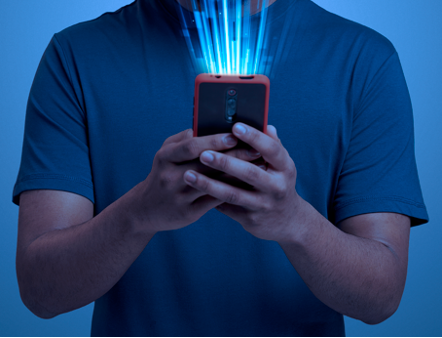
\includegraphics[width=0.4\textwidth]{imgs/fig.png}
    \fonte{Fonte: Freepik (2025).}
\end{figure}

As tabelas são confeccionadas com o objetivo de apresentar resultados numéricos
e valores comparativos tratados estatisticamente e seguem as Normas Tabulares do
IBGE:

\begin{table}[h]
    \centering
    \caption{Exemplo de tabela}
    \label{tab:tabela}
    \setlength{\tabcolsep}{16pt}
    \begin{tabular}{l c c}
        \toprule
        \textbf{Faixa etária} & \textbf{Quantitativo} & \textbf{\%} \\
        \midrule
        17 a 22 anos & 33  & 30   \\
        23 a 28 anos & 93  & 50   \\
        29 a 35 anos & 40  & 10   \\
        36 a 40 anos & 21  & 10   \\
        \midrule
        \textbf{Total} & \textbf{187} & \textbf{100,0} \\
        \bottomrule
    \end{tabular}
    \fonte{IBGE (2012, p. 5).}
\end{table}

Os quadros são identificados por apresentarem dados textuais, o que os
diferencia das tabelas. Devem estar localizados o mais próximo possível do texto
a que se referem e podem ser esquemáticos, comparativos ou descritivos, com ou
sem indicação de dados numéricos. No Quadro \ref{quad:quadro} tem-se um exemplo
de apresentação.

\begin{square}[Exemplo de quadro]
    \label{quad:quadro}
    \renewcommand{\arraystretch}{1.2} % Aumenta o espaçamento entre linhas
    \setlength{\tabcolsep}{10pt} % Ajusta o espaçamento entre colunas
    \begin{tabular}{|l|c|}
        \hline
        \textbf{Gênero Textual} & \textbf{Número de Livros} \\
        \hline
        Poesia   & 12 \\
        \hline
        Romance  & 5  \\
        \hline
        Crônica  & 8  \\
        \hline
        Suspense & 15 \\
        \hline
    \end{tabular}
    \fonte{Dados do Autor (2025).}
\end{square}

\textcolor{blue}{
Dicas: Para construir um referencial teórico, o estudante deve revisar a
literatura, abordando conceitos fundamentais, trabalhos acadêmicos e/ou sistemas
similares ao seu estudo. É essencial incluir trabalhos relacionados, comparando
metodologias e identificando limitações, além de analisar outros sistemas
existentes, destacando suas funcionalidades e diferenciais. A organização do
referencial deve seguir uma progressão lógica, do geral para o específico,
demonstrando a lacuna na pesquisa e  justificando a relevância do estudo.
}

\section{Metologia}

\textcolor{blue}{
Dicas: A Metodologia deve incluir o desenvolvimento do sistema, detalhando sua
implementação de forma clara e objetiva. Caso necessário, os requisitos
funcionais e não funcionais podem ser apresentados para contextualizar o
funcionamento do sistema e justificar as escolhas técnicas. Além disso,
recomenda-se a inclusão de um esquema ilustrativo da arquitetura do sistema,
facilitando a compreensão da sua estrutura e organização. Por fim, é essencial
descrever os métodos de verificação e/ou validação utilizados para garantir a
qualidade do sistema, especificando os critérios adotados para aferir os
aspectos desejados, como desempenho, segurança, usabilidade ou conformidade com
os requisitos definidos.
}

\section{Resultados e Discussão}

\textcolor{blue}{
Dicas: A seção de Resultados e Discussão deve apresentar os dados obtidos na
verificação e/ou validação do sistema, destacando aqueles mais relevantes para
responder às perguntas e atender aos objetivos da pesquisa. A organização dos
resultados deve seguir uma ordem lógica, alinhada à Metodologia, garantindo
clareza na análise. Além de descrever os achados, essa seção deve interpretá-los
e relacioná-los ao referencial teórico, comparando-os com estudos anteriores
para identificar padrões, implicações e possíveis explicações. Gráficos, tabelas
e figuras podem ser utilizados para ilustrar as descobertas de forma objetiva e
facilitar a compreensão. Por fim, a discussão deve contextualizar os resultados,
apontando limitações do estudo, contribuições para a área e direções para
pesquisas futuras, sempre com embasamento nos dados apresentados.
}

\section{Considerações finais}

\textcolor{blue}{
Dias: As considerações finais devem destacar como o trabalho contribui para o
avanço do conhecimento na área, indo além da simples repetição do resumo ou
listagem de resultados. Essa seção deve apresentar uma justificativa científica
clara, indicando a relevância dos achados e suas possíveis aplicações ou
extensões. Além disso, é recomendado sugerir pesquisas futuras e experimentos
complementares que possam aprofundar os resultados obtidos. As conclusões podem
ser tanto gerais quanto específicas, sempre alinhadas aos objetivos
estabelecidos na introdução, garantindo uma síntese coerente e impactante do
estudo \cite{Elsevier2025}.
}

% Referências
\renewcommand{\bibname}{
    \raggedright Referências\vspace{-1.5em}
}
\bibstyle{abntex2-alf}
\bibliography{referencias}

\end{document}
